\section{Tower: from Functions to Architectures}
\label{sec:tower}

In a many embedded systems, programmers produce an entire system of software
that interacts with multiple input and output peripherals concurrently using a
real-time operating system (RTOS). Typical RTOSes provide just a few low-level
locking and signaling primitives for scheduling. Since microcontrollers do not
have virtual memory managment units (MMUs) found on larger processors, the RTOS
kernel can't protect the system against badly behaved user code. These
restrictions put significant burden on the programmer: she must ensure all tasks
and communication between tasks is implemented correctly.

Luckily, we already have Ivory in our toolbox, which guarantees memory-safety of
the generated code. During our initial development of SMACCMPilot, we found
ourselves writing high-quality C functions in Ivory.  But whenever we needed
``glue code'' to implement inter-process communication, initialize
data-structures, read the system clock, lock the processor, etc., we were forced
to abandon our well-typed world and tediously use C directly via Ivory's foreign
function interface.  Furthermore, the hand-written C is OS-specific, meaning it
would have to be rewritten for any OS port.

The hand-written glue code was ruining both our productivity and our assurance
story.  We realized that we could build another EDSL to generate the glue code.
Such an EDSL could be built on ``top of'' Ivory, using Ivory's code-generation
facilities already.  From this idea, the Tower EDSL was born.  In Tower, one
specifies tasks and communication channels that generates correct Ivory
implementations, as well as architecture description artifacts. Tower hides the
dangerous low-level scheduling primitives to the user, and it keeps type
information for channels (i.e. the datatype of the channel message), expressed
as Ivory types, in the Haskell type system.

Tower allows the programmer to describe a static graph of channels and tasks.
This is a restriction of the capabilties of most operating systems, which may
create and destroy tasks or communication datastructures at run-time. However,
for the intended use case in high assurance systems, a static configuration of
channels and tasks makes it easier to reason about memory requirements, and
permits the system to be analyzed for schedulability.

\paragraph{Multiple Interpreters}

%% \begin{figure}
%%   \begin{center}
%% 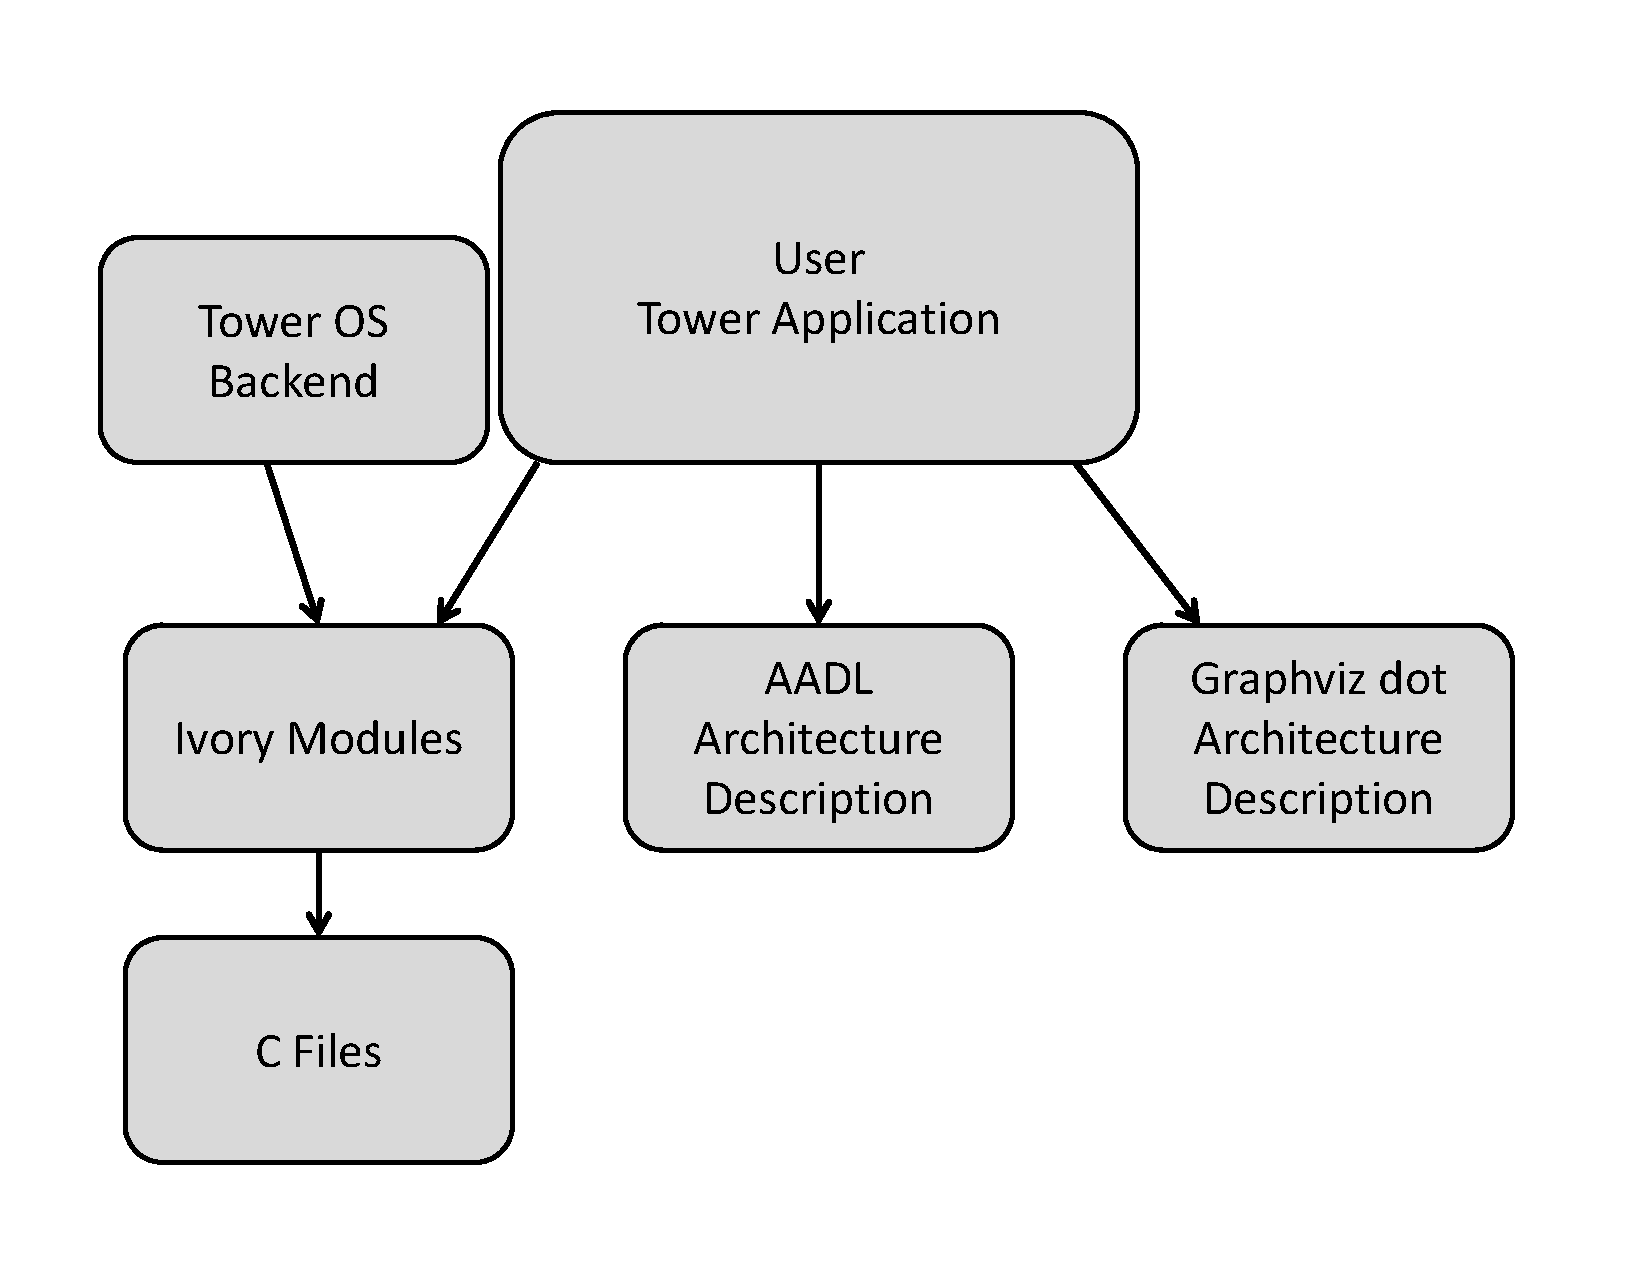
\includegraphics[width=6cm]{figures/tower-artifacts-dia}
%%   \end{center}
%%   \caption[Tower artifacts]{Tower artifact generation.}
%% \label{fig:towerArtifacts}
%% \end{figure}

In the Tower frontend, the programmer specifies a system that can be compiled into
multiple artifacts.

Tower is designed to support different operating systems via a swappable
backend. Since all code that touches operating system primitives is generated by
Tower, it is trivial for the user to specify a system and compile it for
different operating systems. Tower supports both the open-soure
FreeRTOS~\cite{freertos} as well as the formally-verified eChronos
RTOS~\cite{echronos} development by NICTA.

The static tower graph of channels and tasks also makes it possible to
describe the system architecture to external tools. Tower has a backend which
generates a system description in the Architecture Analysis and Design Language
(AADL)~\cite{SAE:AADL}. We also built a backend for the Graphviz dot language.
These output formats make it possible to visualize, analyze, and automatically
check properties about the system, without knowing anything about Haskell,
Ivory, or Tower. This is an important feature when working with teams that may
not all be literate in Ivory/Tower.

